\documentclass[11pt, aspectratio=169]{beamer}

% LuaLaTeXで日本語を使うための必須パッケージ
\usepackage{luatexja}

% 便利な追加パッケージ
\usepackage{booktabs}   % 表の罫線
\usepackage{tikz}       % 図形描画
\usetikzlibrary{decorations.pathreplacing}
\usepackage{graphicx}
\usepackage{hhline}
\usepackage{multirow}
\usetikzlibrary{shapes.symbols, shapes.geometric, arrows.meta, positioning}
\usepackage{listings}   % ソースコード挿入
\lstset{
  basicstyle=\ttfamily\scriptsize,
  frame=single,
  breaklines=true,
  numbers=left,
  numberstyle=\tiny
}

% テーマとカラーテーマの設定
\usetheme{Madrid}
\usecolortheme{orchid}

% ==========================================
% セクション・サブセクションの可視化設定
% ==========================================

% 1. セクション開始時の自動表紙（扉絵）
\AtBeginSection[]{
  \begin{frame}
    \vfill
    \centering
    \begin{beamercolorbox}[sep=8pt,center,shadow=true,rounded=true]{title}
      \usebeamerfont{title}\insertsectionhead\par%
    \end{beamercolorbox}
    \vfill
  \end{frame}
}

% フッターに個別の説明を出すためのマクロ定義
\newcommand{\footertext}[1]{%
  \begin{tikzpicture}[remember picture, overlay]
    % 下端からの距離(yshift)と左端からの距離(xshift)を調整可能
    \node[anchor=south west, font=\footnotesize, text=gray] at ([yshift=1.5ex, xshift=1cm]current page.south west) {#1};
  \end{tikzpicture}%
}

% 2. サブセクション開始時に「現在のセクション内の目次」を自動挿入
\AtBeginSubsection[]{
  \begin{frame}{\insertsectionhead}
    \tableofcontents[currentsection, currentsubsection, subsectionstyle=show/shaded/hide]
  \end{frame}
}

% タイトル情報（hyperrefの警告対策としてオプション引数を追加）
\title{セキュリティプロトコル}
\subtitle{\texttt{SSL/TLS}}
\author[学籍番号: 1280391 / 氏名: 細川夏風]{学籍番号(Student ID): 1280391 \\ 氏名(Name): 細川夏風(Hosokawa Natsuka)}
\institute{高知工科大学(Kochi Univ of Tech)}
\date{\today}

\begin{document}

% TikZスタイル定義
\tikzstyle{client} = [rectangle, rounded corners, draw=blue!60, fill=blue!10, very thick, minimum width=2.5cm, minimum height=1.5cm, align=center]
\tikzstyle{server} = [rectangle, rounded corners, draw=green!60!black, fill=green!10, very thick, minimum width=2.5cm, minimum height=1.5cm, align=center]
\tikzstyle{internet} = [cloud, cloud puffs=12, cloud puff arc=120, aspect=2, draw=gray, fill=gray!10, very thick, minimum width=3.5cm, minimum height=2cm, align=center]
\tikzstyle{arrow} = [-{Stealth[scale=1.2]}, thick, draw=black!80]

% タイトルスライド
\begin{frame}
    \titlepage
\end{frame}

% 目次スライド
\begin{frame}{目次}
    \tableofcontents
\end{frame}

% ==========================================
% ここから本文
% ==========================================
\section{自己紹介}
\begin{frame}{自己紹介}
  \begin{columns}[T]
    \begin{column}{0.48\textwidth}
      高知工科大学 情報学群 学士$3$年 \\
      所属研究室: シカール研究室

      \vspace{1.5em}

      \begin{description}[研究:]
        \item[研究:] \texttt{SAGIN}という新構想ネットワークの無線妨害の緩和手法
        \item[趣味:] 家で作ったネットワーク環境をいじってアプリ開発とかハニーポッド作って遊んだり，音楽で\texttt{Jazz}をやったりもしてます．映画とかも好きで一番好きな映画は「インターステラー」です！
      \end{description}
    
    \end{column}
    \begin{column}{0.48\textwidth}
      \begin{figure}
        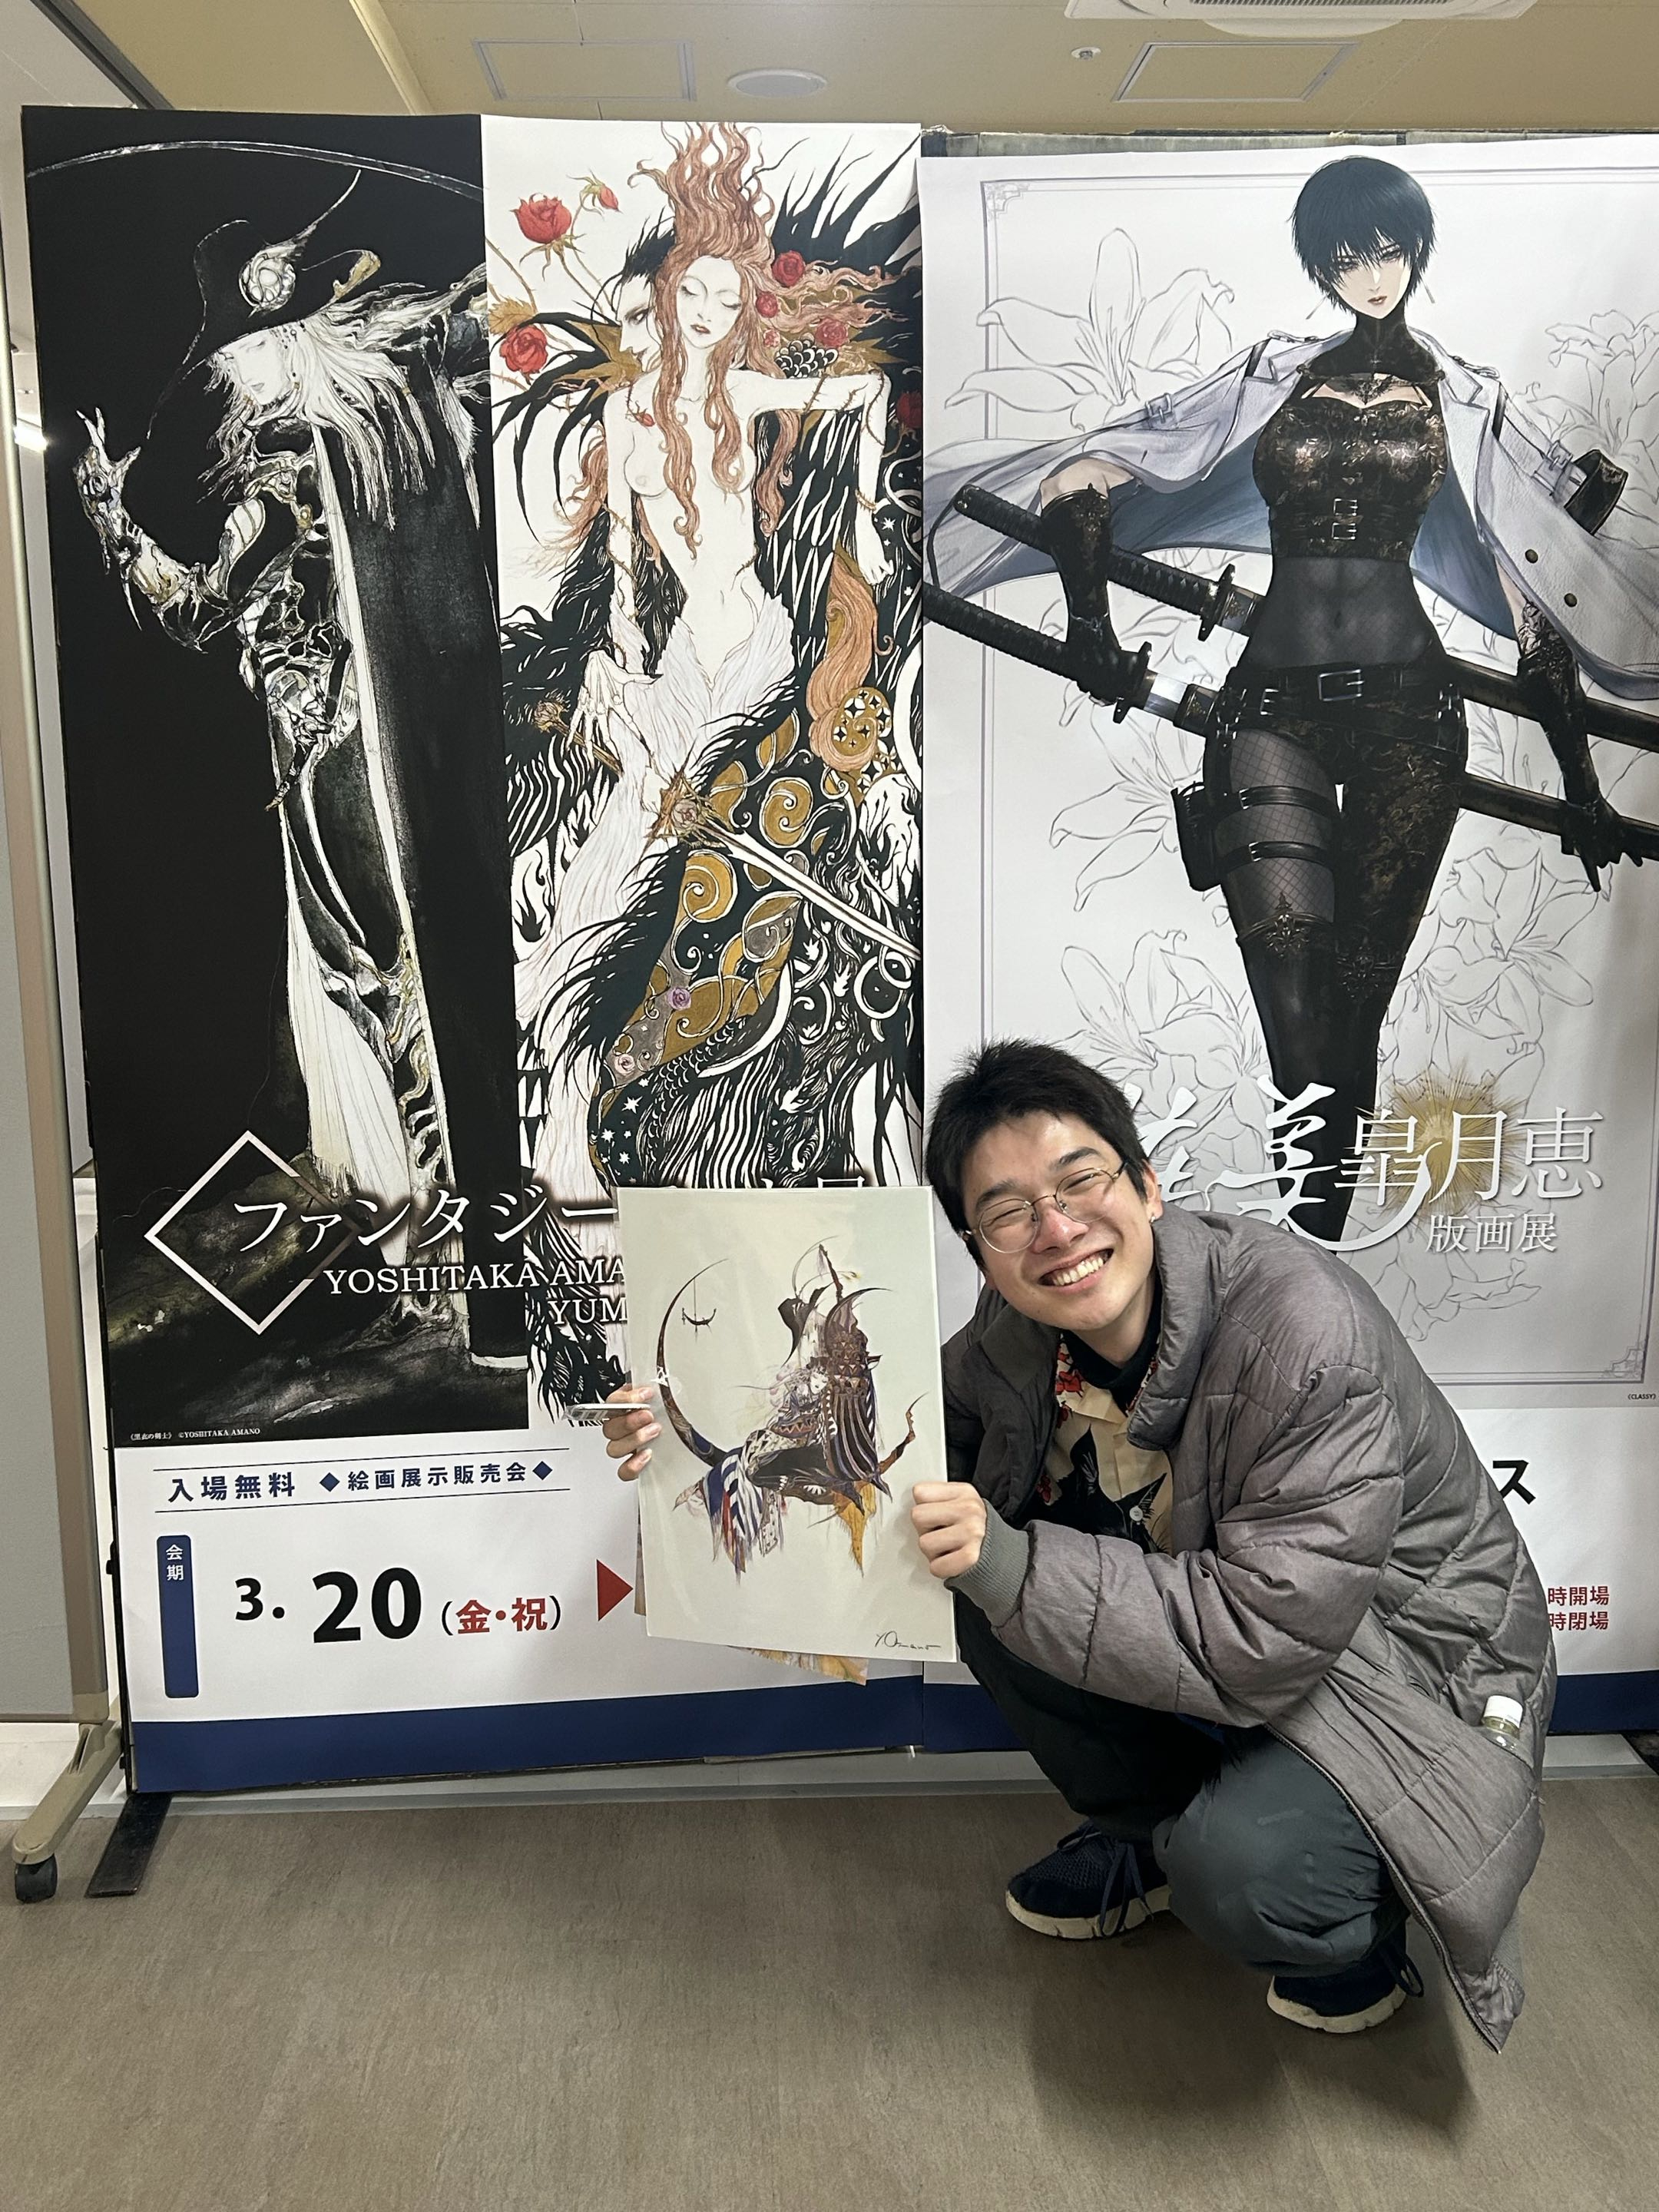
\includegraphics[width=0.55\linewidth]{Myself.jpg}
        \caption{好きな画家の絵を買えてニコニコの僕}
      \end{figure}
    \end{column}
  \end{columns}
\end{frame}

\section{セキュリティプロトコル}

\subsection{セキュリティプロトコルについて}
\begin{frame}{セキュリティプロトコルについて}
    % ここに内容を記述
  \begin{columns}
    \begin{column}{0.48\textwidth}
      \begin{alertblock}{通信の脅威}
        \begin{itemize}
          \item 盗聴
          \item 改竄
          \item ハイジャック
          \item なりすまし
          \item 捏造
          \item 再送
        \end{itemize}
      \end{alertblock}
    \end{column}
    \begin{column}{0.48\textwidth}
      \begin{block}{通信を安全に行うための技術}
        \begin{itemize}
          \vspace{0.8em}
          \item 公開鍵暗号方式
          \item 共通鍵暗号方式
          \item 鍵交換方式
          \item メッセージの改竄検知
          \item 認証プロトコル
          \vspace{0.8em}
        \end{itemize}
      \end{block}
    \end{column}
  \end{columns}
  \vspace{0.5em}
  セキュリティプロトコルはこれらの脅威に対して，右の技術を適切に組み合わせ用いる事によって\texttt{CIA}の確保を目指している．
\end{frame}

\begin{frame}{利用場面とプロトコルの種類}
  \begin{table}[htbp]
    \centering
    \caption{セキュリティプロトコルの利用場面と種類}
    \begin{tabular}{|c|c|c|} \hline
      \texttt{OSI}層 & 名称 & 概要 \\ \hhline{|=|=|=|}
      アプリケーション層 & \texttt{S/MIME} & 電子メールの暗号化とディジタル署名のプロトコル \\ \hline
      アプリケーション層 & \texttt{SSH} & 遠隔ログインのプロトコル \\ \hline
      トランスポート層 & \texttt{SSL/TLS} & \texttt{Web}通信などの様々な暗号化で利用されるプロトコル \\ \hline
      ネットワーク層 & \texttt{IPsec} & \texttt{IP}パケット自体を保護対象とするプロトコル \\ \hline
      データリンク層 & \texttt{L2TP} & 暗号器機能がないので\texttt{IPsec}などと併用される \\ \hline
    \end{tabular}
  \end{table}
\end{frame}

\subsection{よりセキュアな通信}
\begin{frame}{よりセキュアな通信}
  \begin{itemize}
    \item \texttt{\textbf{E2EE(End-to-End Encryption)}} \\
      \texttt{E2EE}はメッセージアプリケーションなどにおいて，通信の当事者同士のみが閲覧可能である2点間の暗号方式のこと．
    \item \textbf{前方秘匿性} \\
      前方秘匿性は，もし仮に暗号が危殆化してしまった場合にそれまでに行われた通信の安全性を保証する性質のこと．
    \item \texttt{\textbf{PCS(Post-Conpromise Security)}} \\
      \texttt{PCS}は暗号方式が危殆化してもその後，ある程度は安全性を保証する概念のこと．ラチェット機構と呼ばれる仕組みで使用している鍵を変化させて通信を行うため，暗号が危殆化してもある程度の安全性は保証される．
  \end{itemize}
\end{frame}

\section{\texttt{SSL/TLS}の概要}

\begin{frame}{\texttt{SSL/TLS}の概要}
  \begin{itemize}
    \item \textbf{\texttt{SSL(Secure Socket Layer)}} \\
      \texttt{SSL}は暗号化，認証，改竄検知などを行うセキュリティプロトコルである．これまでバージョンが$1,2,3$と更新されてきた．      
     \item \textbf{\texttt{TLS(Transport Layer Security)}} \\
       \texttt{SSL ver:3.0}以降の$1999$年に\texttt{RFC}$2246$にて新たなセキュリティプロトコルである\texttt{TLS}が策定された．その後，\texttt{UDP}上で\texttt{TLS}を実現する\texttt{DTLS}も策定割れた．

  \end{itemize}
  \begin{alertblock}{\texttt{SSL}の使用について}
    $1996$年以降の\texttt{ver.}$3.0$から更新はされておらず，非推奨となっており，現在はほとんどのブラウザで使用されていない．それでもこの名前が用いられることが多いのは慣習の部分が大きいからだと思われる．
  \end{alertblock}
\end{frame}

\begin{frame}{\texttt{SSL/TLS}の構造}
  \begin{figure}
    \centering
    \begin{tabular}{|p{2.2cm}|p{2.2cm}|p{2.2cm}|p{2.2cm}|}
      \hline
      \textbf{Handshake} \newline \tiny 共有状態を確立 & \textbf{ChangeCipherSpec} \newline \tiny 切り替え通知 & \textbf{Alert} \newline \tiny 異常を通知 & \textbf{アプリケーション} \\
      \hline
      \multicolumn{4}{|c|}{\textbf{Record}} \\
      \multicolumn{4}{|c|}{\tiny 暗号化されたアプリケーションデータをはじめSSL/TLSでやりとりされるデータを扱うプロトコル} \\
      \hline
      \multicolumn{4}{|c|}{\textbf{TCP}} \\
      \hline
    \end{tabular}
    \caption{\texttt{SSL/TLS}の構造図}
  \end{figure}
\end{frame}

\section{\texttt{SSL/TLS}のプロトコル詳細}

\subsection{\texttt{Record}プロトコル}

\begin{frame}{\texttt{Recode}プロトコル}
  \texttt{SSL/TLS}のすべての通信は，送信するデータを最大$2^{14}$バイト以下のフラグメントに分ける．それらを個別に暗号化するなどして，受信者側に送信する．受信者はこの工程と逆の工程を行う．この手順の定義を行っているのが\texttt{Record}ぷろとこるである．

  送信者は計算した\texttt{MAC}値を添付し，暗号化し，ヘッダを追加する．この作成されたフラグメントのことを``\textbf{\texttt{record}}''という．実際にはこの``\textbf{\texttt{record}}''を送り合ってやり取りを行う．この際，シーケンス番号が``\texttt{record}''にはつけられているため，順序の検知が可能である．

\begin{figure}[b]
  \centering
    \begin{tikzpicture}[scale=0.8, transform shape]
      % 全体の送信データ用の上部ブレース
      \draw [decorate,decoration={brace,amplitude=6pt},thick] (0, 1.5) -- (13.2, 1.5);
      \node[above=6pt] at (6.6, 1.5) {\textbf{送信するデータ}};

      % --- 1つ目のレコード ---
      % Recordヘッダ
      \draw[thick, fill=white] (0, 0) rectangle (1.8, 0.9);
      \node[align=center] at (0.9, 0.45) {\scriptsize Record\\[-2pt]\scriptsize ヘッダ};

      % データフラグメント (グレー塗りつぶし)
      \draw[thick, fill=gray!30] (1.8, 0) rectangle (5.2, 0.9);
      \node at (3.5, 0.45) {\small データフラグメント};

      % MAC (グレー塗りつぶし)
      \draw[thick, fill=gray!30] (5.2, 0) rectangle (6.5, 0.9);
      \node at (5.85, 0.45) {\small MAC};

      % レコード全体のブレース (下)
      \draw [decorate,decoration={brace,amplitude=5pt,mirror},thick] (0,-0.1) -- (6.5,-0.1);
      \node[below=6pt] at (3.25,-0.1) {\small レコード};

      % 暗号化部分のブレース (さらに下)
      \draw [decorate,decoration={brace,amplitude=4pt,mirror},thick] (1.8,-0.9) -- (6.5,-0.9);
      \node[below=6pt, align=center] at (4.15,-0.9) {\scriptsize 暗号化されたデータと\\[-2pt]\scriptsize 暗号化されたMAC};

      % --- 省略記号 ---
      \node at (7.3, 0.45) {\large $\dots$};

      % --- 2つ目のレコード ---
      \begin{scope}[xshift=8.1cm]
        % Recordヘッダ
        \draw[thick, fill=white] (0, 0) rectangle (1.8, 0.9);
        \node[align=center] at (0.9, 0.45) {\scriptsize Record\\[-2pt]\scriptsize ヘッダ};

        % データフラグメント
        \draw[thick, fill=gray!30] (1.8, 0) rectangle (3.8, 0.9);
        \node at (2.8, 0.45) {\small データ};

        % MAC
        \draw[thick, fill=gray!30] (3.8, 0) rectangle (5.1, 0.9);
        \node at (4.45, 0.45) {\small MAC};

        % レコード全体のブレース (下)
        \draw [decorate,decoration={brace,amplitude=5pt,mirror},thick] (0,-0.1) -- (5.1,-0.1);
        \node[below=6pt] at (2.55,-0.1) {\small レコード};

        % 暗号化部分のブレース (さらに下)
        \draw [decorate,decoration={brace,amplitude=4pt,mirror},thick] (1.8,-0.9) -- (5.1,-0.9);
        \node[below=6pt, align=center] at (3.45,-0.9) {\scriptsize 暗号化されたデータと\\[-2pt]\scriptsize 暗号化されたMAC};
      \end{scope}

    \end{tikzpicture}
    \caption{\texttt{record}のデータ処理}
  \end{figure}
\end{frame}

\begin{frame}{\texttt{Record}プロトコル(\texttt{Record}ヘッダ)}
  \texttt{Record}ヘッダには，以下の$3$種類のフィールドがある．
  \begin{block}{\texttt{Record}ヘッダのフィールド}
    \begin{itemize}
      \item \texttt{length} \\
        フラグメント化する前の平文全体のサイズ．最大$2^{14}$を一塊として送受信する．
      \item \texttt{SSL version} \\
        通信に使用する\texttt{SSL}のバージョン．
      \item \texttt{content type}
        メッセージの種類を示したもの．$4$種類のタイプがサポートされている．
    \end{itemize}
  \end{block}
\end{frame}

\subsection{\texttt{Handshake}プロトコル}

\begin{frame}{\texttt{Handshake}プロトコル}
  \texttt{Handshake}プロトコルの目的はお互いが等しく暗号アルゴリズムや暗号鍵などを等しく保持し，暗号通信に必要な共有状態を確立することである．暗号通信を行うために送受信者で合意して置かなければならない合意情報の組み合わせを``暗号スイート''という．

\vspace{1em}

  \texttt{Handshake}にはいくつかの種類がある．
  \begin{itemize}
    \item サーバー認証モード: \texttt{RSA}や\texttt{DSS}を用いてサーバを認証する方式
    \item クライアント認証モード: さらいにクライアントとサーバが相互に認証する方式
  \end{itemize}

  一般的にはサーバー認証モードが使われるが，よりセキュアなものにしたい場合はクライアント認証モードが使われることがある．
\end{frame}

\begin{frame}{\texttt{Handshake}プロトコル(メッセージ): サーバ認証モード}
  \begin{itemize}
    \item \textbf{Hello Request}: クライアントは新たな方式での通信の合意のメッセージ
    \item \textbf{Client Hello}: クライアントが通信の開始を通知し，対応可能な暗号方式やランダム数を送信する．
    \item \textbf{Server Hello}: サーバーが使用する暗号方式などを決定して返信する．
    \item \textbf{Certificate}: サーバーのデジタル証明書を送信し，クライアントが検証する（\textbf{サーバー認証}）．
    \item \textbf{Server Key Exchange / Hello Done}: 鍵共有用のパラメータや，サーバー側のメッセージ送信終了を通知する．
    \item \textbf{Client Key Exchange}: クライアントが鍵共有データを送信し，共通の秘密鍵を生成する．
    \item \textbf{Change Cipher Spec \& Finished}: お互いに暗号通信への切り替えとハンドシェイクの完了を確認し合う．
  \end{itemize}
\end{frame}

\begin{frame}{\texttt{Handshake}プロトコル(メッセージ): クライアント認証モード}
  \begin{itemize}
    \item \textbf{Client Hello}: クライアントが通信の開始を通知し，対応可能な暗号方式やランダム数を送信する．
    \item \textbf{Server Hello}: サーバーが使用する暗号方式などを決定して返信する．
    \item \textbf{Certificate}: サーバーのデジタル証明書を送信し，クライアントが検証する（\textbf{サーバー認証}）．
    \item \textbf{Server Key Exchange / Certificate Request / Hello Done}: 鍵共有パラメータや終了通知に加え，サーバーからクライアントへ証明書の提示を要求する．
    \item \textbf{Client Certificate / Client Key Exchange}: クライアント自身の証明書送信と鍵共有データの送信を行う．
    \item \textbf{Certificate Verify}: クライアントが秘密鍵の所持を証明する署名を送信する（\textbf{クライアント認証}）．
    \item \textbf{Change Cipher Spec \& Finished}: お互いに暗号通信への切り替えとハンドシェイクの完了を確認し合う．
  \end{itemize}
\end{frame}

\section{\texttt{TLS}}

\subsection{\texttt{TLS}$1.3$}
\begin{frame}{\texttt{TLS}$1.3$の概要}
  \texttt{version}$1.2$から\texttt{version}$1.3$になったことによっていくつかの改善があった．
  \begin{block}{変更点}
    \begin{itemize}
      \item 利用可能な暗号スイートの変更 \\
      \begin{itemize}
        \item \texttt{TLS\_AES\_128\_CCM\_SHA256}: \texttt{AEAD}は\texttt{AES\_128\_CCM}，\texttt{HKDF}のハッシュ関数は\texttt{SHA256}
        \item \texttt{TLS\_AES\_128\_CCM\_8\_SHA256}: \texttt{AEAD}は\texttt{AES\_128\_CCM\_8}，\texttt{HKDF}のハッシュ関数は\texttt{SHA256}
        \item \texttt{TLS\_AES\_128\_GCM\_SHA256}: \texttt{AEAD}は\texttt{AES\_128\_GCM}，\texttt{HKDF}のハッシュ関数は\texttt{SHA256}
        \item \texttt{TLS\_AES\_256\_GCM\_SHA384}: \texttt{AEAD}は\texttt{AES\_256\_GCM}，\texttt{HKDF}のハッシュ関数は\texttt{SHA385}
        \item \texttt{TLS\_CHACHA20\_POLY1305\_SHA256}: \texttt{AEAD}は\texttt{CHACHA20\_POLY1305}，\texttt{HKDF}のハッシュ関数は\texttt{SHA256}
      \end{itemize}
      \item \texttt{Handshake}の\texttt{1-RTT}化 \\
        通信開始時に送る暗号スイートの候補リストからの返事をもらうだけの\texttt{1RTT}化に成功
    \end{itemize}
  \end{block}
\end{frame}

\subsection{\texttt{DTLS}}
\begin{frame}{\texttt{DTLS}の概要}
  \texttt{TLS}は\texttt{TCP}を想定して作れられているプロトコルであるため，そのままに\texttt{UDP}上で動かすことは難しい．その問題はメッセージを単位フラグメントあたりでは復号ができないため損失や順序に問題がなく届く必要がある．
  
  そのために以下のような修正が行われている．
  \begin{block}{修正内容}
    \begin{itemize}
      \item \texttt{Handshake}の修正: 確認用返答メッセージとタイマーによる返答確認時間の導入
      \item \texttt{record}の修正:
      \begin{itemize}
        \item 複数のコネクション識別のための\texttt{epoch}フィールドの追加
        \item シーケンス番号の確認のための\texttt{sequence\_number}の追加
      \end{itemize}
    \end{itemize}
  \end{block}
\end{frame}

\begin{frame}{セキュリティ対策}
  \textbf{再送攻撃対策} \\
    \texttt{DTLS}には，シーケンス番号があるため，再送攻撃を防ぐことが可能である．

  \vspace{1em}

  \textbf{\texttt{DoS}攻撃対策} \\
    この問題の解決のためには\texttt{IPsec}でも用いられるステートレスクッキー(\texttt{Stateless cookie})という技術を用いている．最初の通信にステートレスクッキーを生成し，それを添付して通信を行う．今後はそれを認証することによって通信を維持していく．
\end{frame}
     
\end{document}

